% Created 2026-04-23 Thu 12:08
% Intended LaTeX compiler: lualatex
\DocumentMetadata{lang = en-US,pdfversion = 2.0,pdfstandard = ua-2,tagging = on,tagging-setup = {math/setup=mathml-SE},}
\documentclass[11pt]{article}
\usepackage{amsmath}
\usepackage{fontspec}
\usepackage{graphicx}
\usepackage{longtable}
\usepackage{wrapfig}
\usepackage{rotating}
\usepackage[normalem]{ulem}
\usepackage{capt-of}
\usepackage{hyperref}
\usepackage[margin=1in]{geometry}
\usepackage{fontspec}
\usepackage{verbatim, multicol, tabularx,}
\usepackage{amsmath, amsthm, amssymb, stmaryrd, latexsym, bm, listings, qtree}
\usepackage{framed}
\usepackage{xcolor,colortbl}
\usepackage{media9}
\usepackage[export]{adjustbox}
\usepackage{algorithm}
\usepackage[noend]{algpseudocode}
\usepackage{tikz,pgfplots}
\usetikzlibrary{shapes.geometric}
\let\oldquote=\quote
\let\endoldquote=\endquote
\colorlet{shadecolor}{cyan!15}
\renewenvironment{quote}{\begin{shaded*}\begin{oldquote}}{\end{oldquote}\end{shaded*}}
% From https://tex.stackexchange.com/questions/7032/good-way-to-make-textcircled-numbers
\newcommand*\circled[1]{\tikz[baseline=(char.base)]{\node[shape=circle,draw,inner sep=2pt] (char) {#1};}}
\DeclareMathOperator*{\argmin}{arg\!min}
\DeclareMathOperator*{\argmax}{arg\!max}
\lstset{frame=tb, aboveskip=1mm, belowskip=0mm, showstringspaces=false, columns=flexible, basicstyle={\scriptsize\ttfamily}, numbers=left, frame=single, breaklines=true, breakatwhitespace=true}
\hypersetup{colorlinks=true,urlcolor=blue}
\usepackage{tagpdf}
\tagpdfsetup{activate-all}
\tagpdfsetup{math/alt/use}
\usepackage{polyglossia}
\setdefaultlanguage[variant=en-US]{english}
\author{Christopher Simpkins}
\date{Kennesaw State University}
\title{Artificial Intelligence\\\medskip
\large Knowledge Representation}
\hypersetup{
 pdfauthor={Christopher Simpkins},
 pdftitle={Artificial Intelligence},
 pdfkeywords={},
 pdfsubject={Artificial Intelligence Knowledge Representation},
 pdfcreator={Emacs 30.2 (Org mode 9.7.11)}, 
 pdflang={English}}
\begin{document}

\maketitle
\section{Ontological Engineering}
\label{sec:org10d966b}


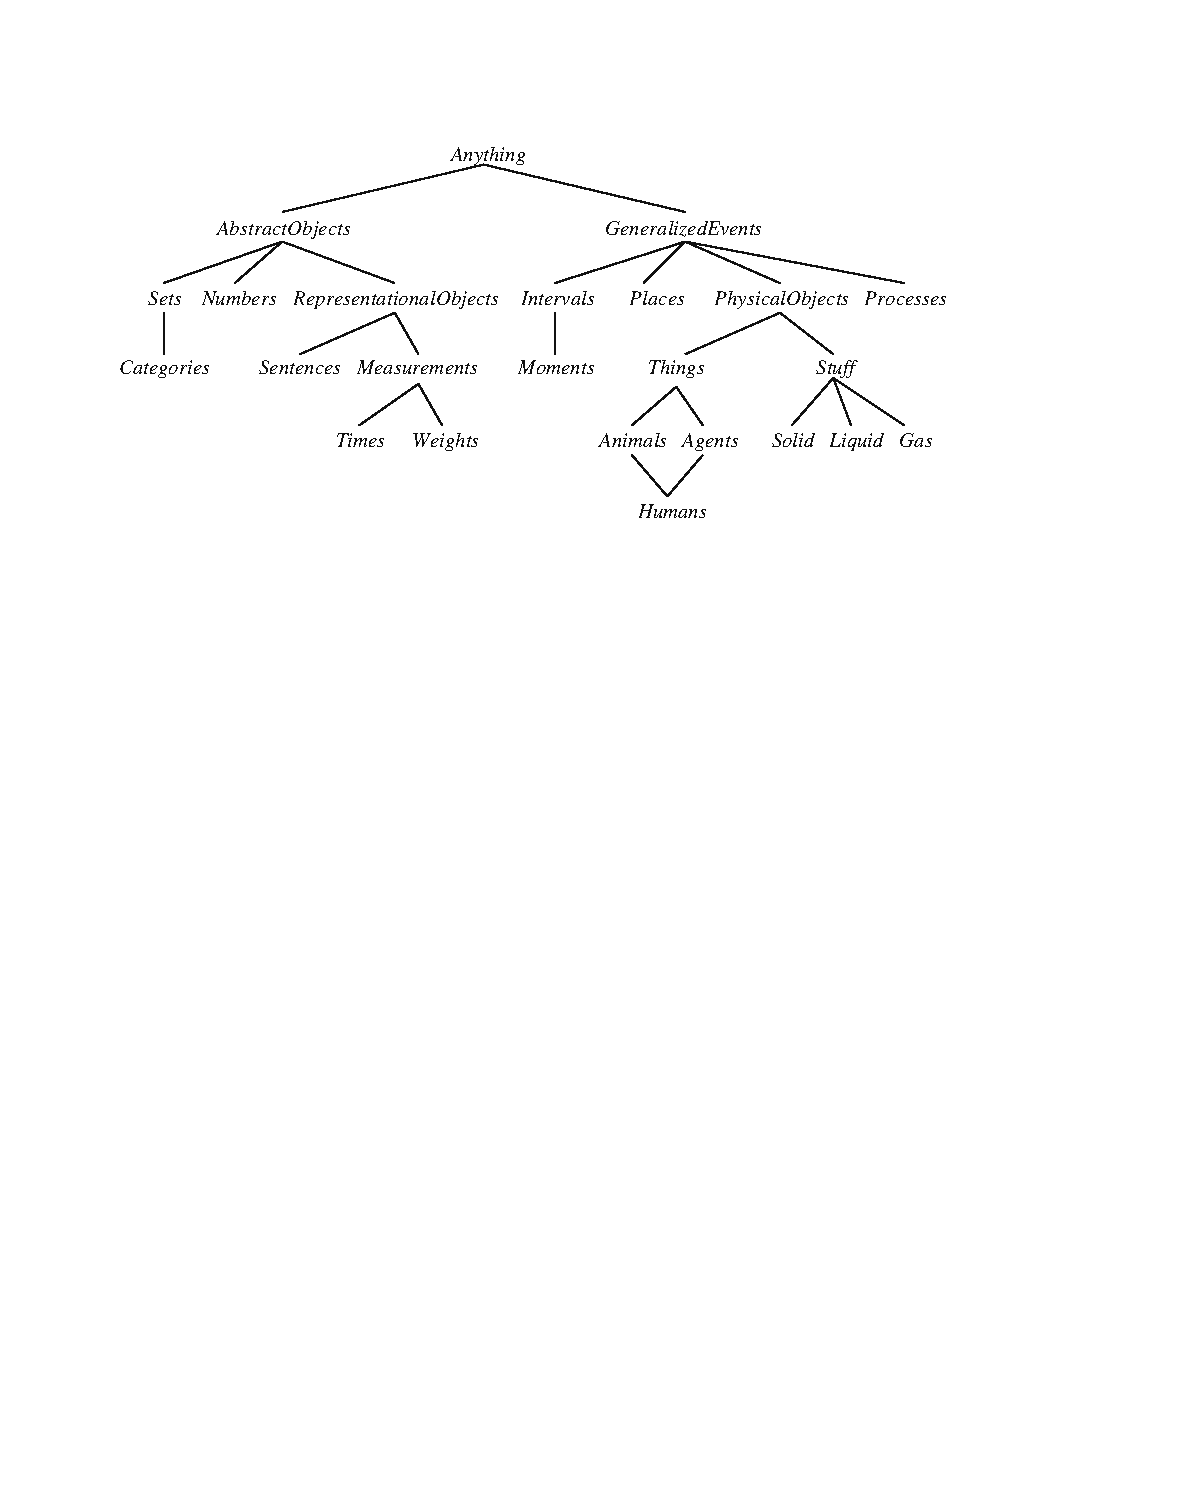
\includegraphics[alt={aima fig 10_01 upper ontology world},height=2.8in]{aima-fig-10_01-upper-ontology-world.pdf}
\section{Categories and Objects}
\label{sec:orgc8afc1d}

Foo
\section{Events}
\label{sec:org52416d9}


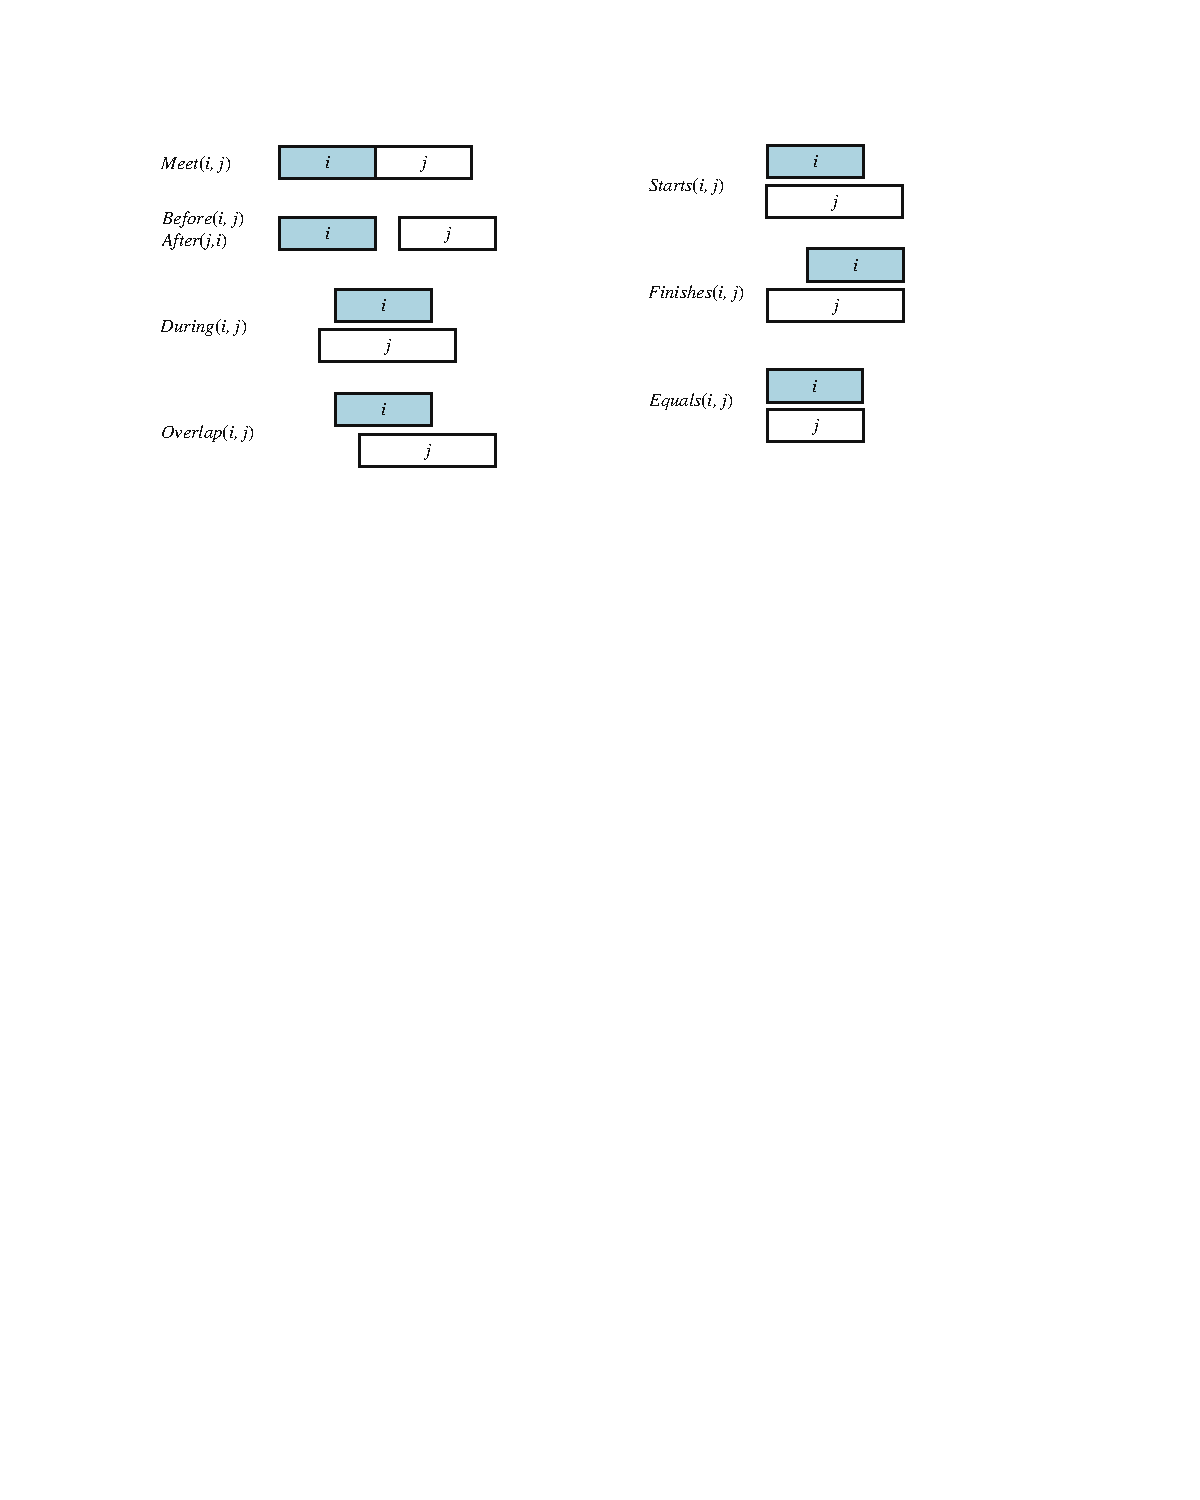
\includegraphics[alt={aima fig 10_02 predicates time intervals},height=2.8in]{aima-fig-10_02-predicates-time-intervals.pdf}
\section{Fluents}
\label{sec:orgbe55ced}


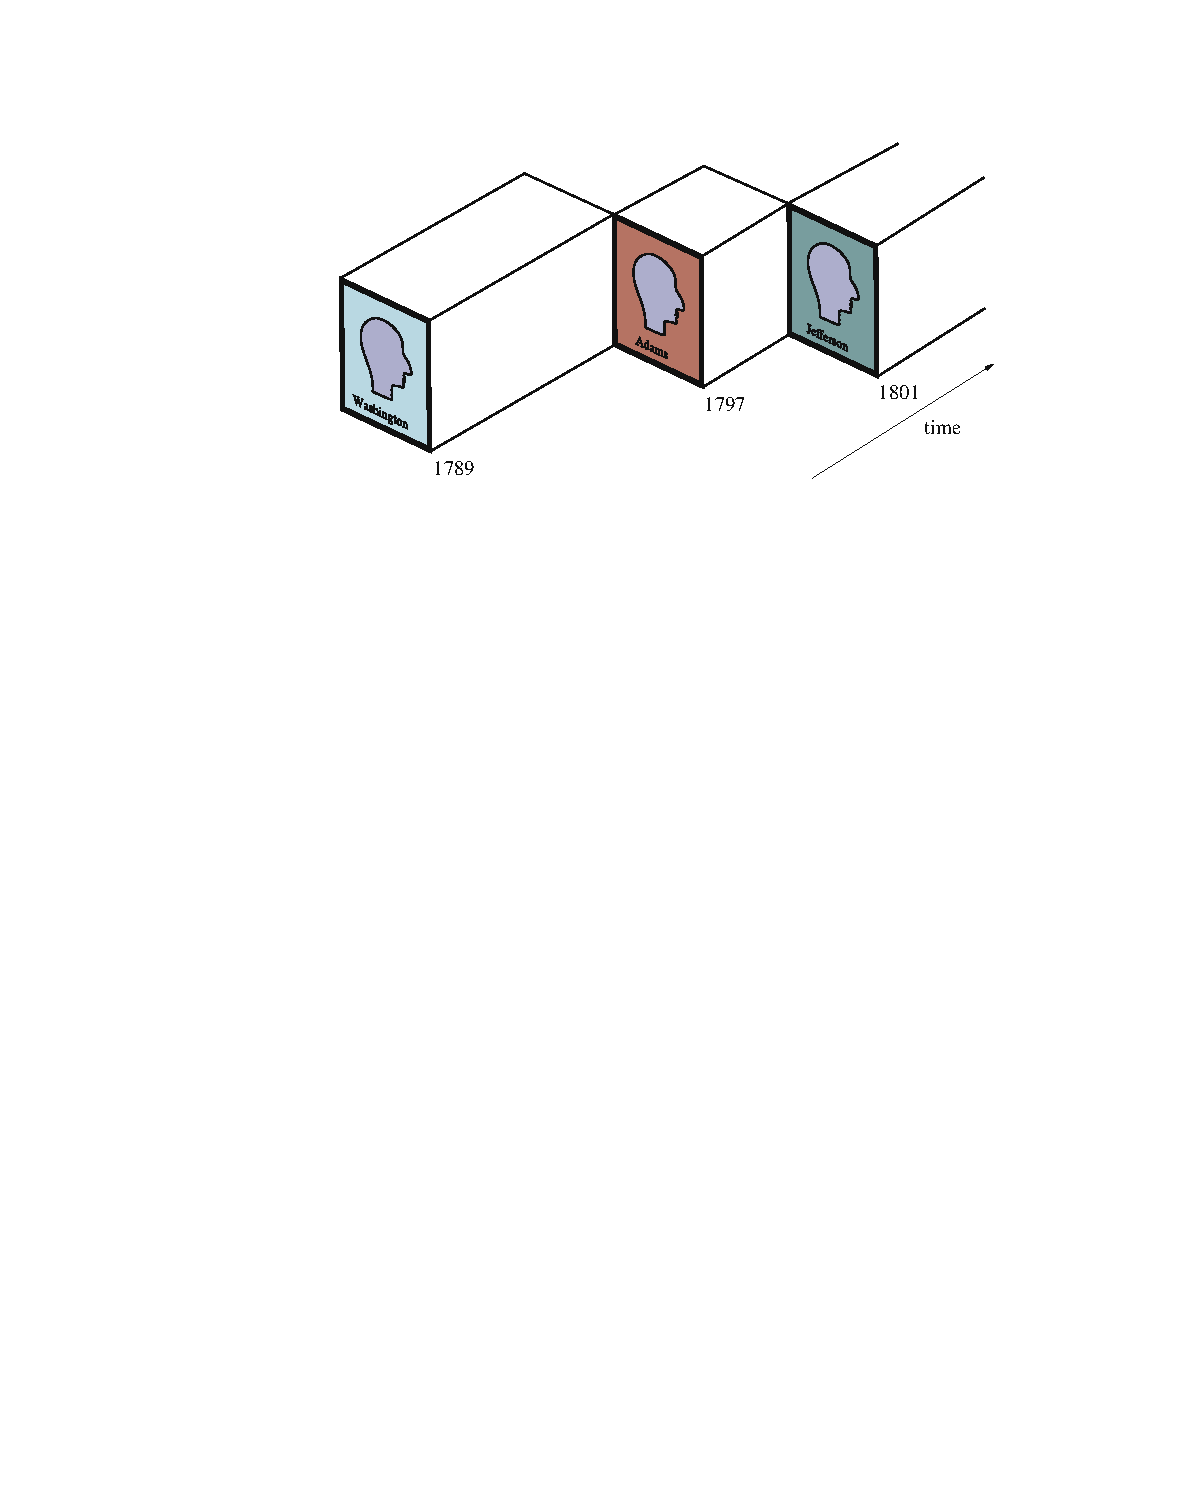
\includegraphics[alt={aima fig 10_03 schematic object president},height=2.8in]{aima-fig-10_03-schematic-object-president.pdf}
\section{Mental Objects and Modal Logic}
\label{sec:org56b3d56}

Foo
\section{Reasoning Systems for Categories}
\label{sec:orgcf377b9}


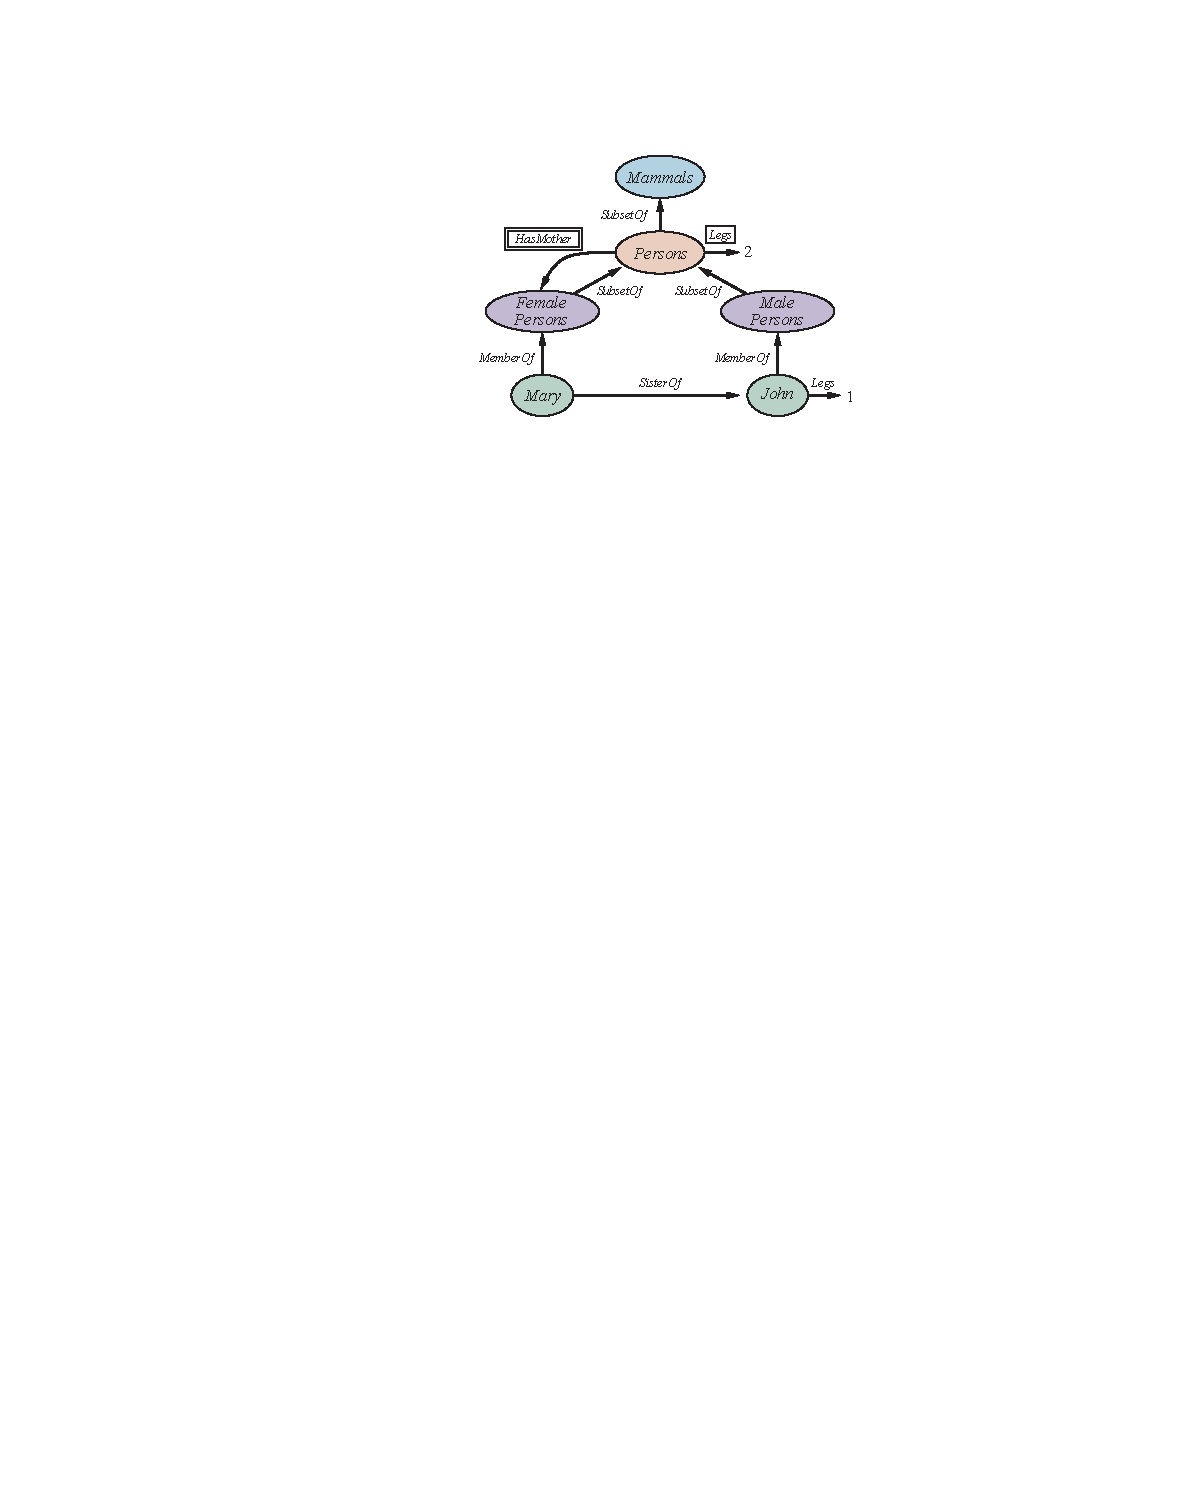
\includegraphics[alt={aima fig 10_04 semantic network 4 objects},height=2.8in]{aima-fig-10_04-semantic-network-4-objects.pdf}
\section{Reasoning Systems for Categories}
\label{sec:org796abea}


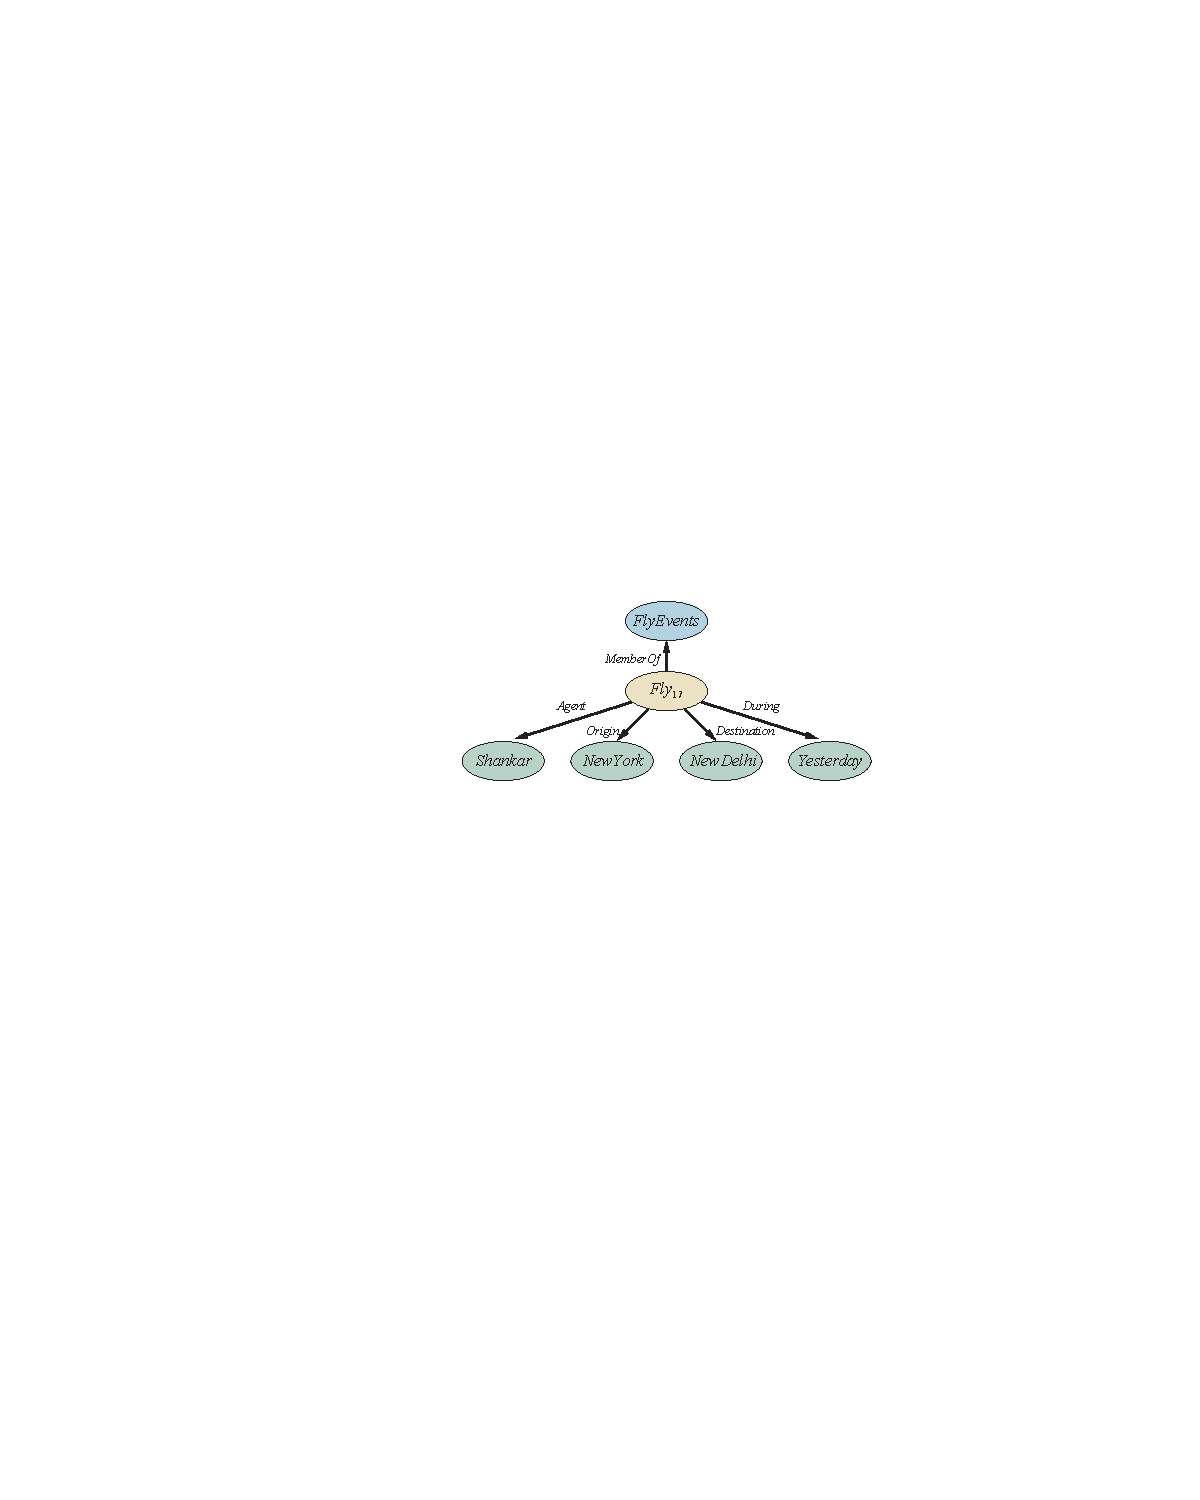
\includegraphics[alt={aima fig 10_05 semantic network assertion fly event},height=2.8in]{aima-fig-10_05-semantic-network-assertion-fly-event.pdf}
\section{Description Logics}
\label{sec:org17612ae}


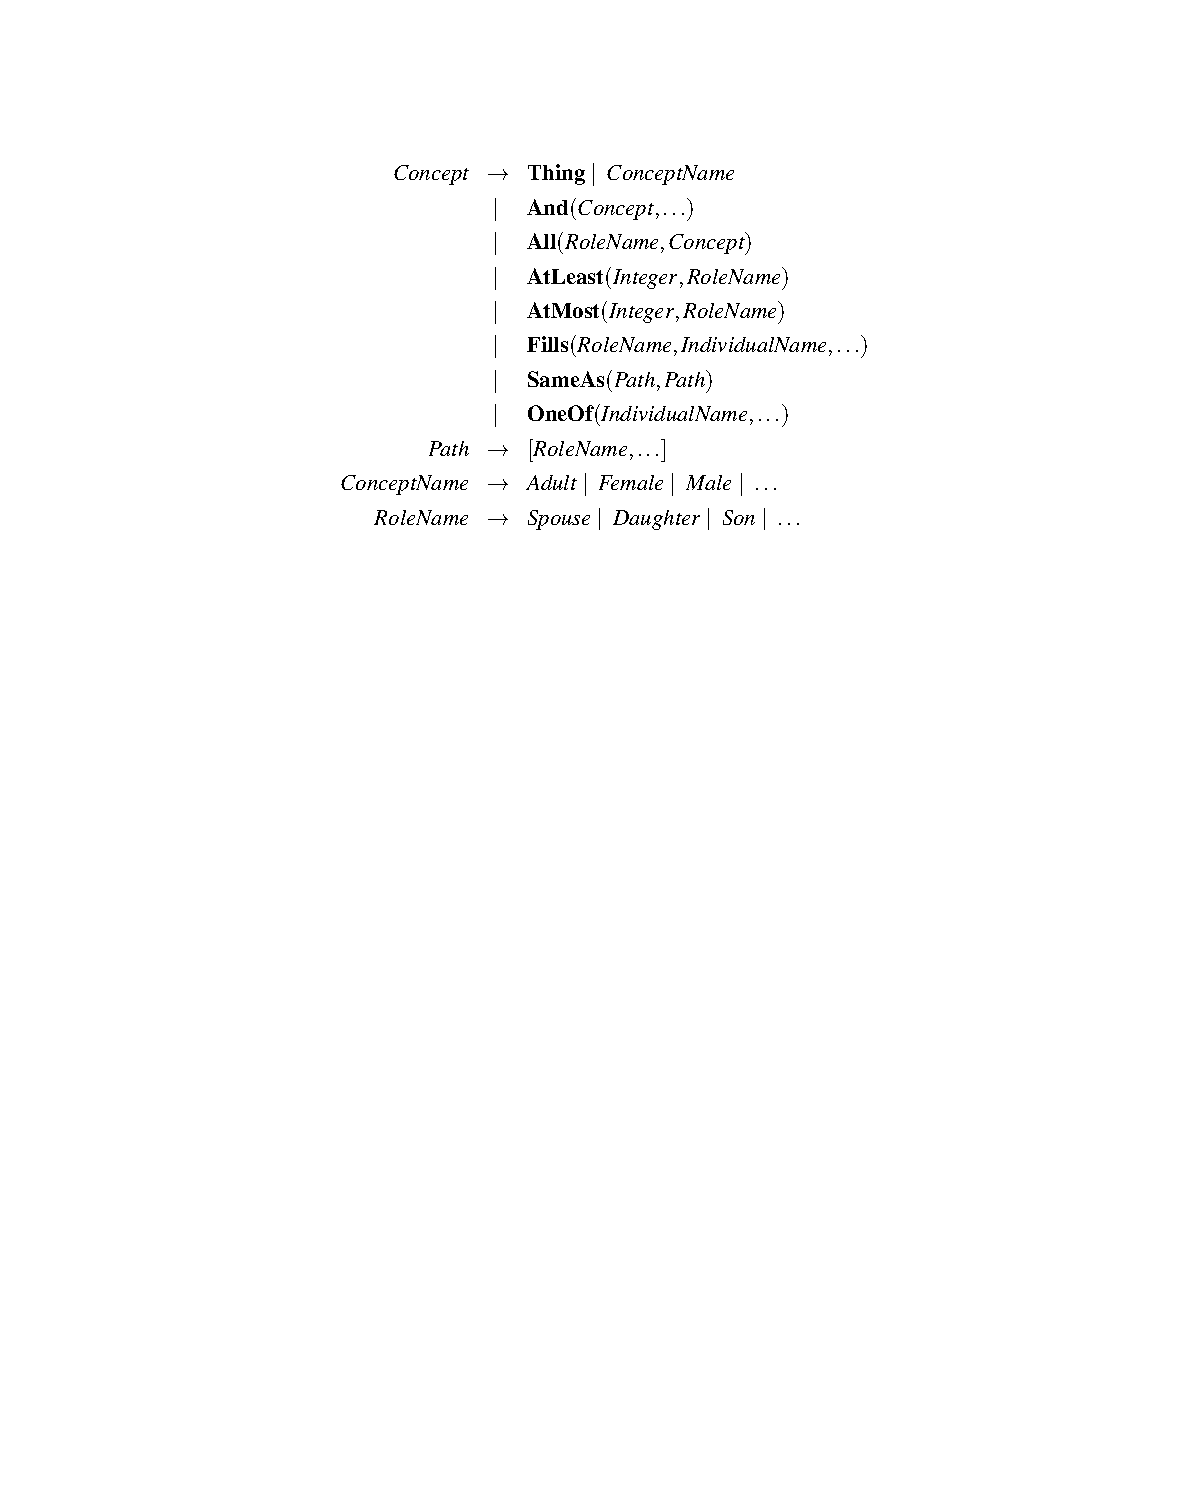
\includegraphics[alt={aima fig 10_06 syntax of classic description logic},height=2.8in]{aima-fig-10_06-syntax-of-classic-description-logic.pdf}
\section{Reasoning with Default Information}
\label{sec:org5a6ab2b}

Truth maintenance systems
\end{document}
